As we are interested in understanding the potential energy savings and RH improvement across continental US, we need the weather data collected from major cities across the continent with resolution smaller than every hour. The ISD-lite dataset made available by NOAA (National Oceanographic Association of America) provides air temperature, relative humidity and geographic location at weather stations across major city centers and airports across continental US. This data is publicly available on NOAA’s ftp server. We downloaded a total of 13,800 files for the monitored weather in 2018 for the purpose of this analysis. Since the climate zones, as we are plotting in Figure~\ref{fg:stations}. 

\begin{figure}[h!]
\centering
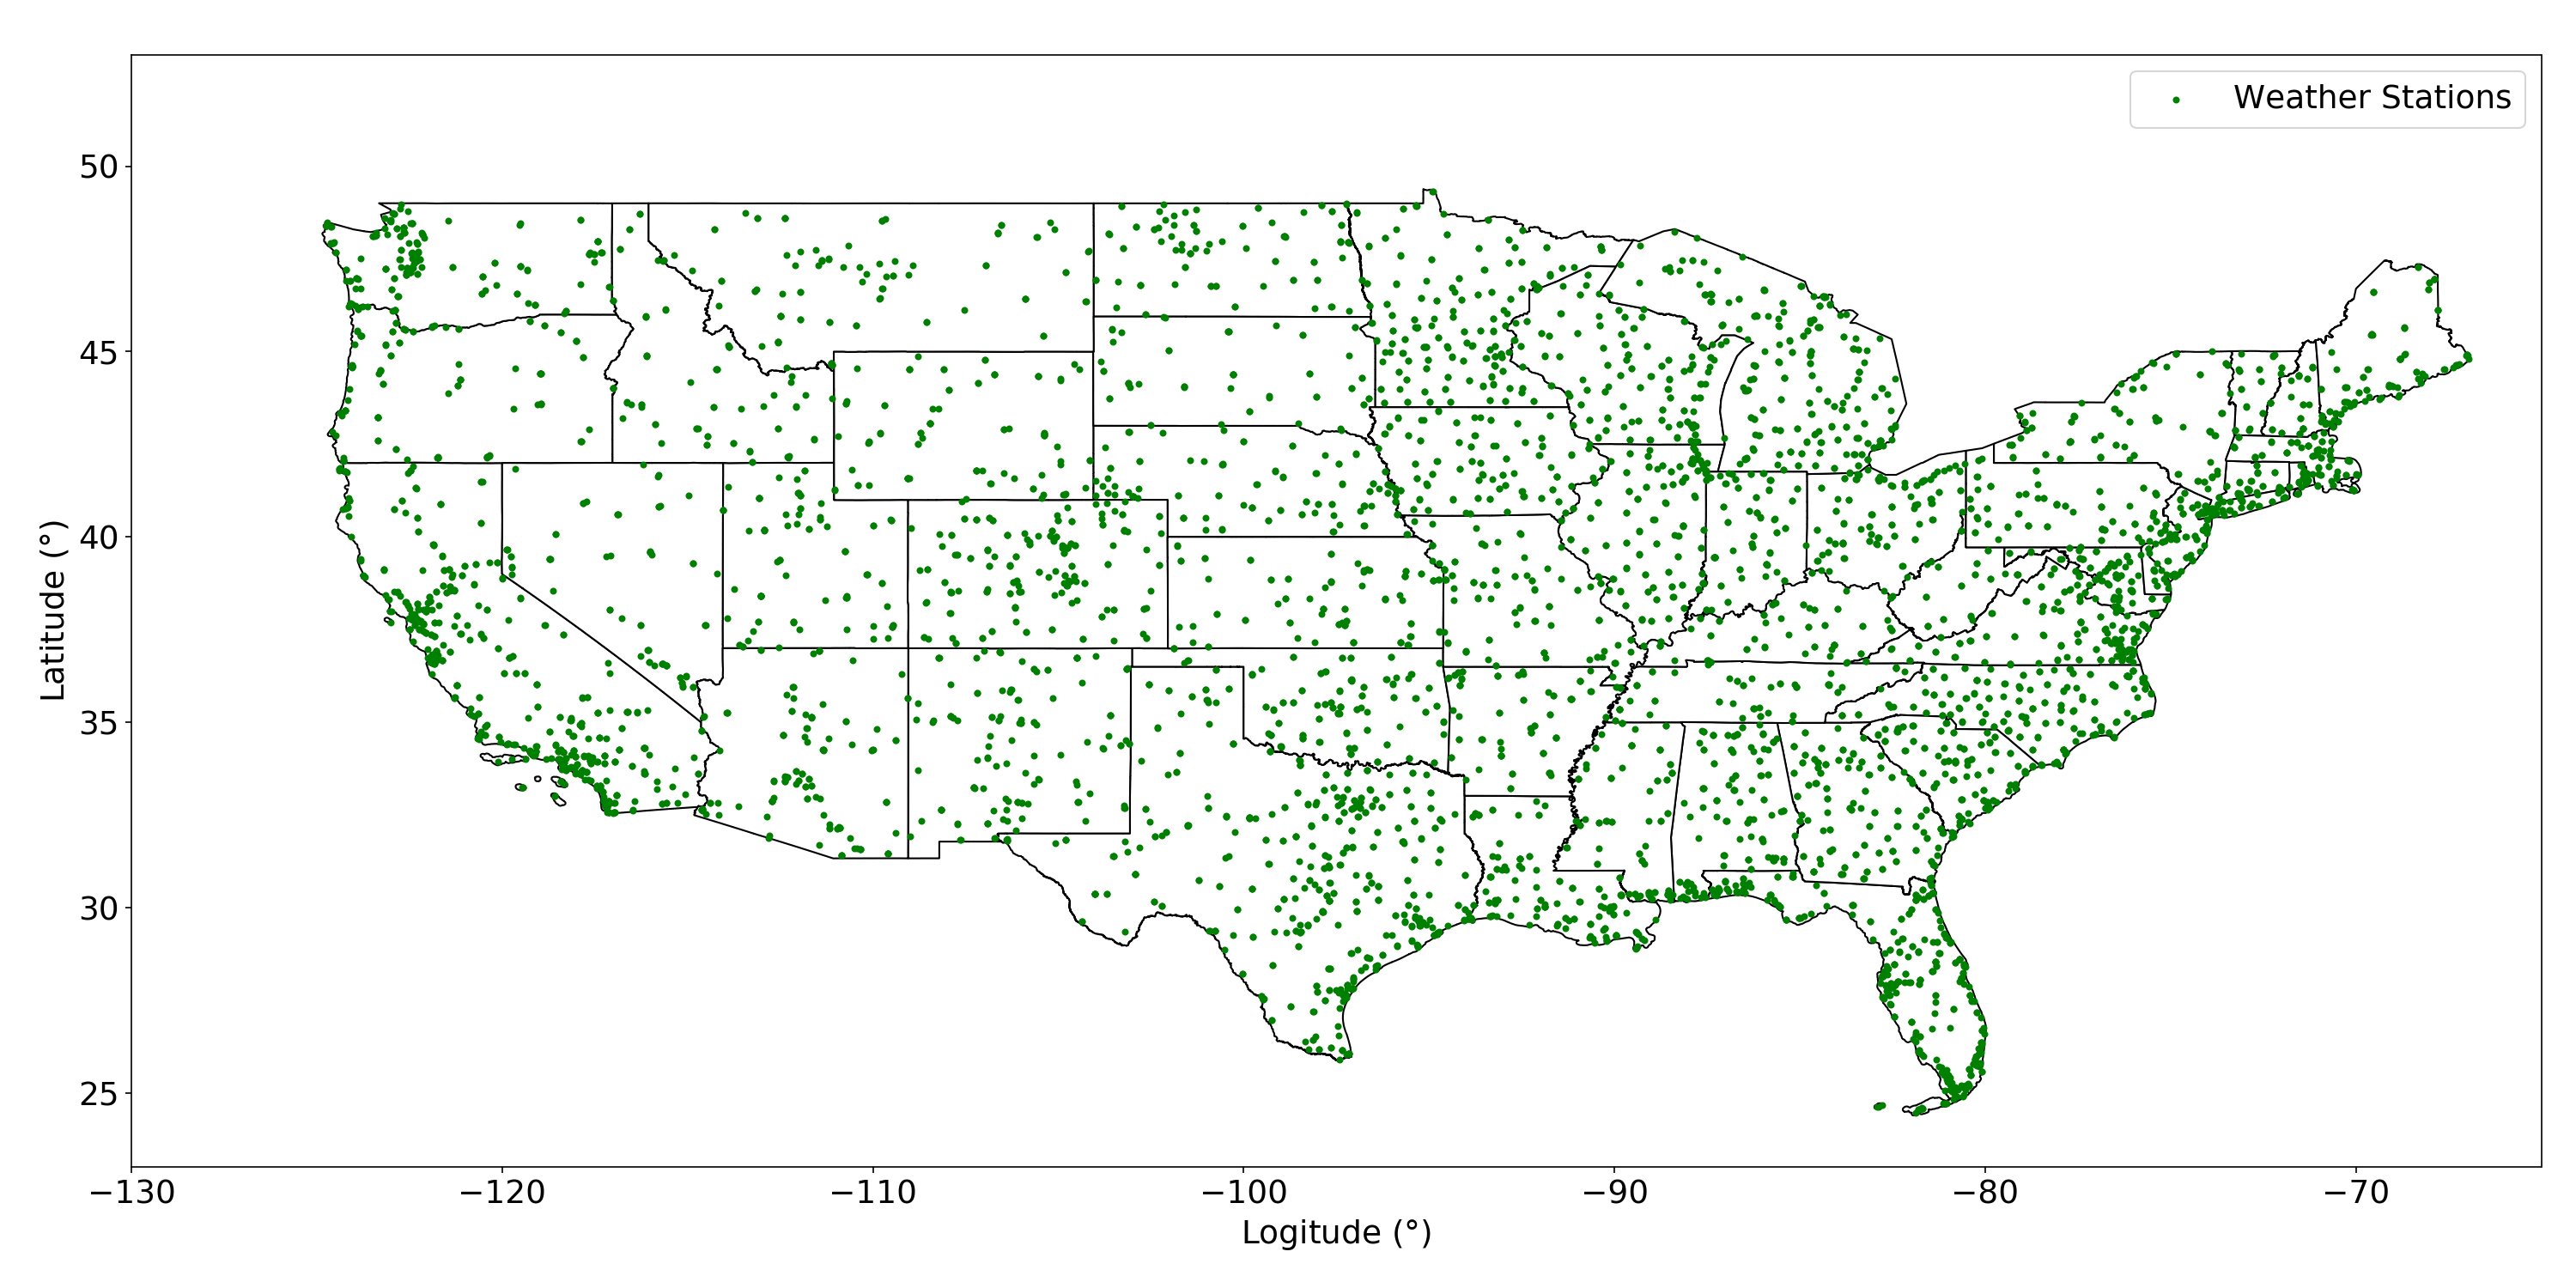
\includegraphics[width=\textwidth]{stations.png}
\caption{Locations of climate station files clipped to the USGS geometry in NOAA ISD-lite, 2017.}\label{fg:stations}
\end{figure}

Upon scraping the NOAA ftp server for the 2018 weather files, we used the pandas data frame library in Python to clean up and regroup the files into time-stamped weather data, and re-sampled on an hourly rate. We also used the CoolProps library to calculate the enthalpy of moist air at different states, and appended the resulting hourly enthalpy states. The resulting weather files will therefore have the air temperature, relative humidity, specific enthalpy for 8760 hours in 2018 across all the stations. We are plotting an example of the data collected in one of the weather stations in Figure~\ref{fg:sampleh}.


\begin{figure}
\centering
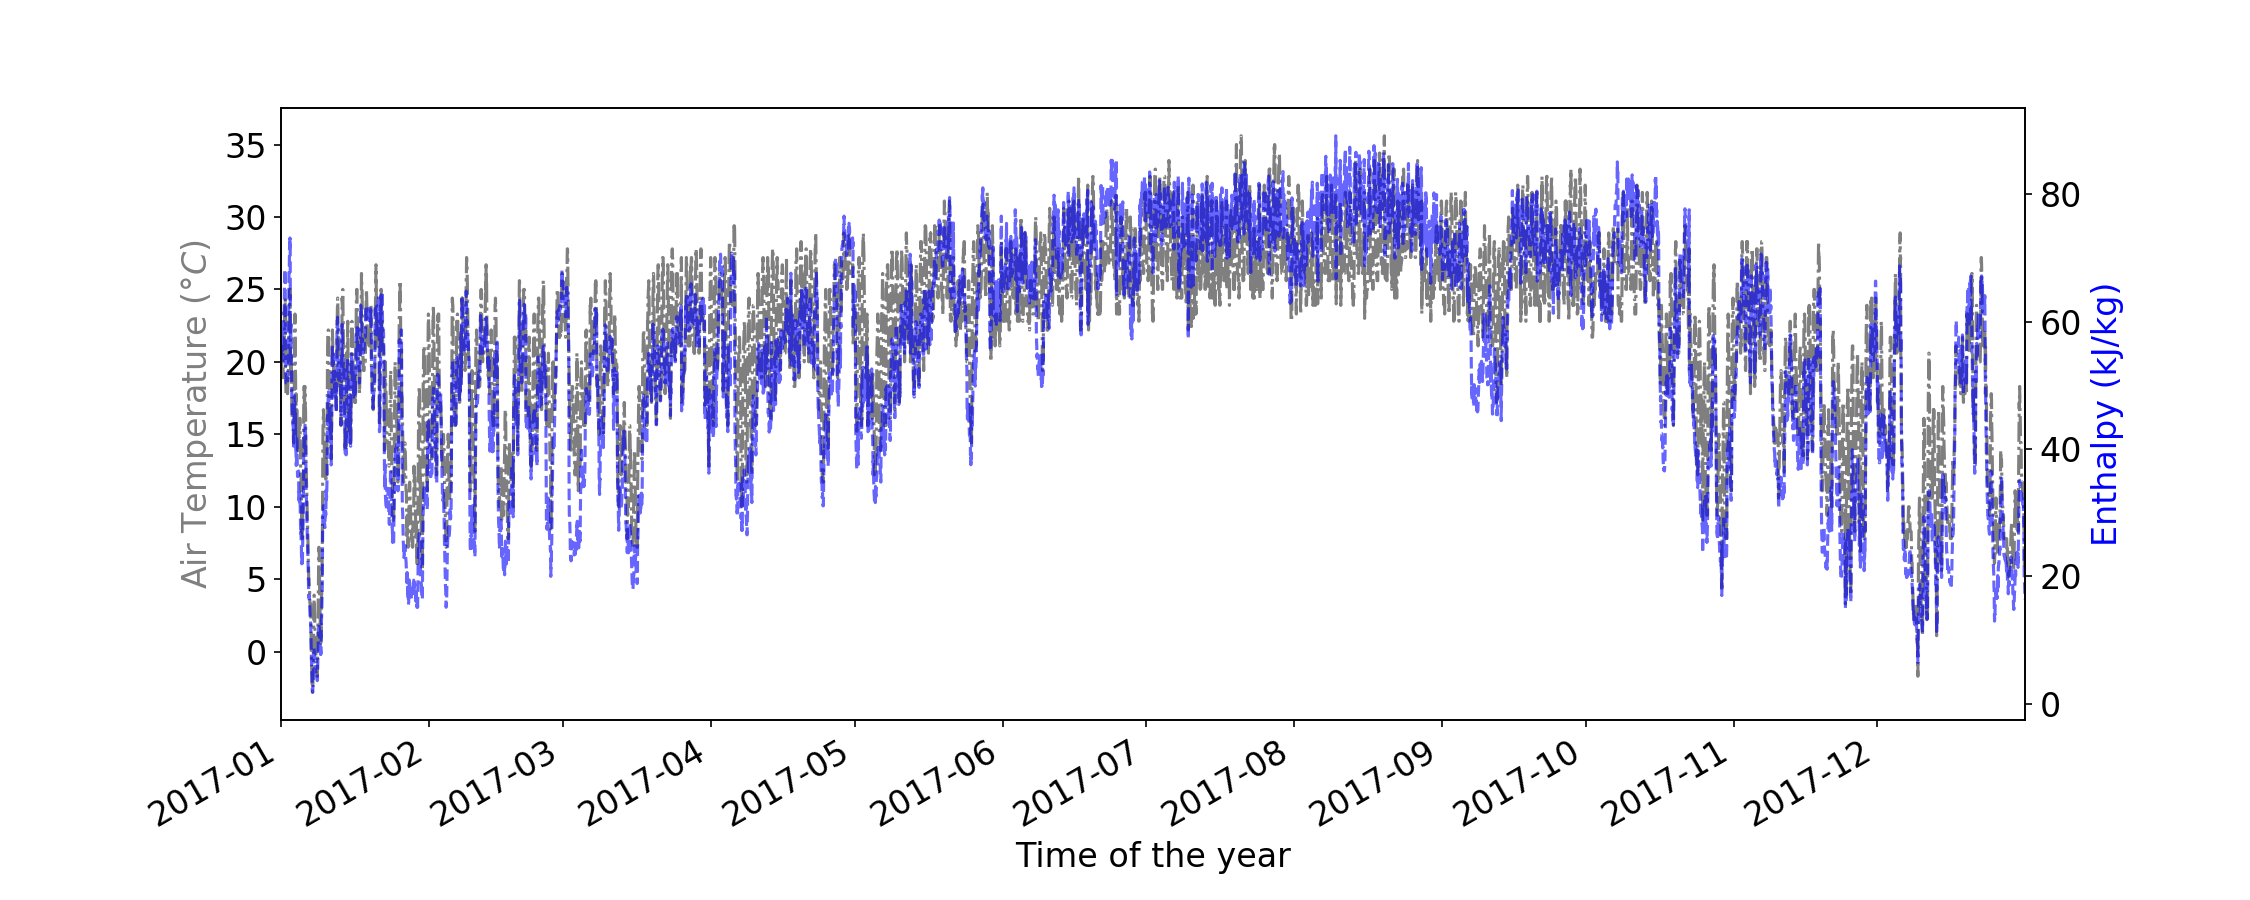
\includegraphics[width=\textwidth]{tbd_h.png}
\caption{ Processed Outdoor Dry-bulb temperature against outdoor specific enthalpy for the weather station in Station ID.}\label{fg:sampleh}
\end{figure}


We will primarily divide our analysis into two parts. The first part focuses on the energy savings of the cooling scenario and the RH improvements for the average heating/cooling condition for the weather stations. We will plot this as heat maps that can be generated from the weather files analyzed. 
%Heating, RH improvements (bad to good) very visual, can use previous plots until we have new ones generated. We're only running this as preliminary improved analysis. Do ew mark out TODOs?
For the heating scenario, we estimate how changing the set point may result in improvements in the RH through a spatial plot of four cases of set points and their resulting RHs across all the weather station we identified. This allows us to estimate the resulting RH distribution from the weather data we collected throughout the continental US. We created an illustration as shown in Figure~\ref{fg:process} to explain how we processed the data, and how it's connected to different levels of analysis.. %Spatial comparison of four temperature states. Figure needs updating.

Operating under the second stage of hypothesis where there are additional humidifiers for home units, we also estimate the potential energy savings in the latent loads that no longer has to be satisfied by comparing the room air enthalpies. These energy savings can be estimated for the daily average to generate an overall year-round enthalpy comparison and categorized into binned plots for both the heating and the subsequent cooling cases. 
%Cooling, energy savings, percentage? For different climates? Bin the results? You wouldn't be able to read it... energy reduction maps. 
For the cooling scenario, we estimate the latent energy savings potential by comparing the overall energy demand in all-air systems against radiant system. 

\begin{figure}[h!]
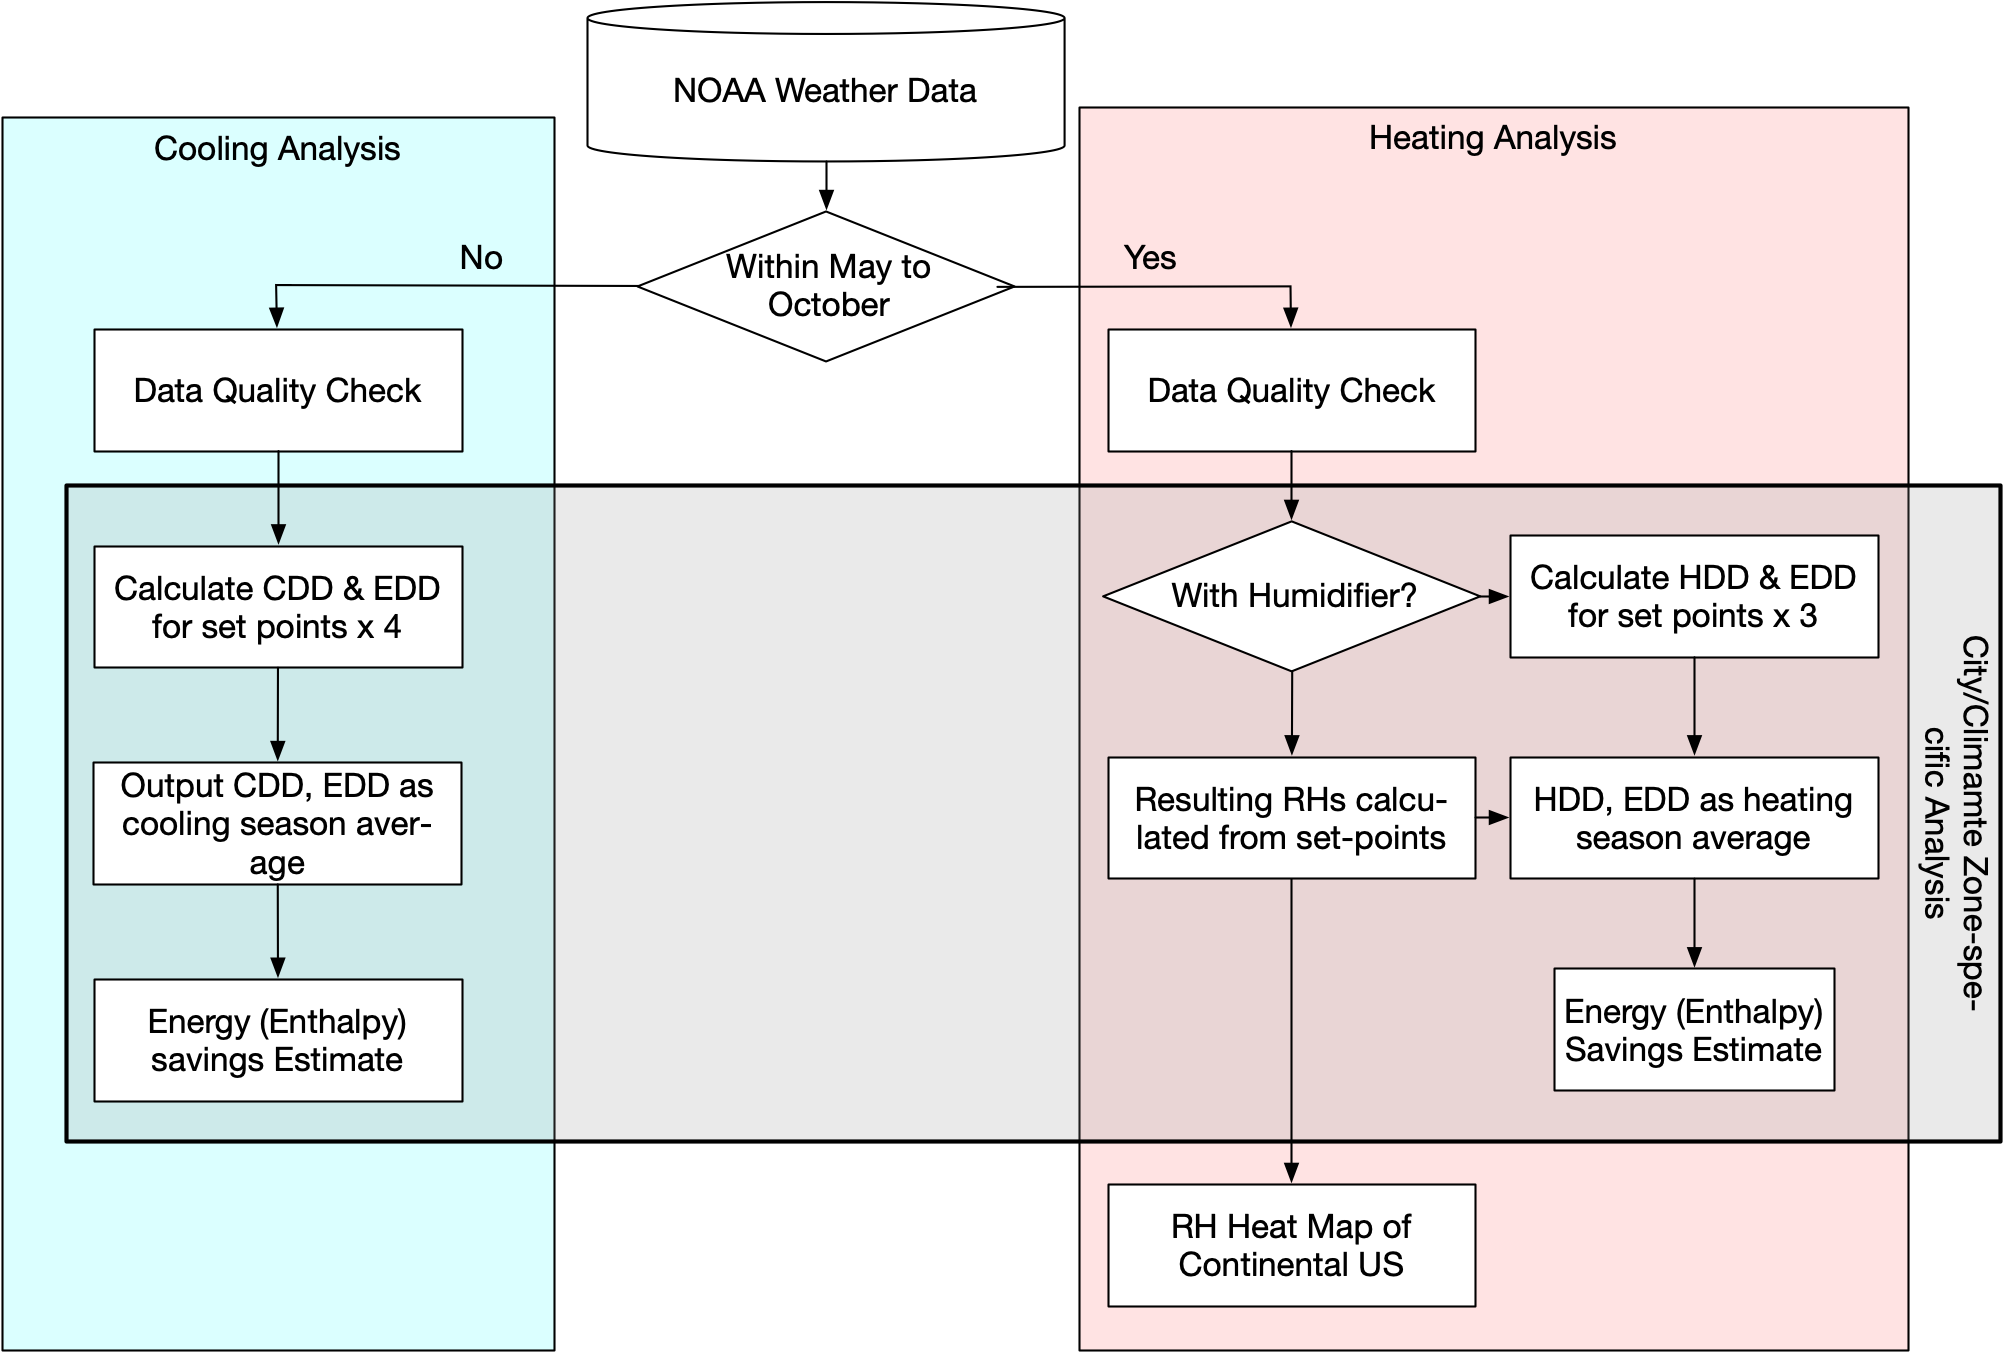
\includegraphics[width=\textwidth]{diagram_radhum}
\caption{Processing of NOAA weather data in relation to the heating and cooling scenarios for daily and hourly (city-specific) data analysis.}\label{fg:process}
\end{figure}

We also hope to identify temporally how the resulting RH and energy consumption may vary, particularly for different climate zones. We will examine this through analyzing selected time series as examples of different climate zones. The cities selected for respective climate zones are listed as the followings in Table~\ref{tab:cities}.

        \begin{table}[h!]
        \centering
        \resizebox{0.9\textwidth}{!}{%
        \begin{tabular}{l|lllllll}
        Climate Zone  & City          & State             & Latitude  & Longtitude & Air Temperature (\degree C)& Relative Humidity(\%)\\\hline
        1 & Miami         & Florida           & +25.788  & -80.317    & 16.51 & 82.28\\
        2 & New Orleans   & Louisiana         & +29.997  & -90.278    & 14.11 & 76.85\\
          & Houston       & Texas             & +29.717  & -95.383    & 14.35 & 66.50\\
          & Austin        & Texas             & +30.395  & -97.567    & 12.75 & 67.77\\
        3 & El Paso       & Texas             & +31.811  & -106.376   & 12.07 & 40.26\\
          & Atlanta       & Georgia           & +33.912  & -84.941    & 11.75 & 70.05\\
        4 & Washington DC & Virginia/Maryland & +38.935  & -77.447    & 9.55  & 63.40\\
          & Philadelphia  & Pennsylvania      & +39.873  & -75.227    & 8.62  & 62.02\\
          & Seattle       & Washington        & -122.314 & +112.8     & 16.86 & 71.65\\
        5 & Denver        & Colorado          & +39.833  & -104.658   & 7.22  & 53.85\\
        6 & Minneapolis   & Minnesota         & +44.883  & -93.229    & 4.70  & 67.44\\
        7 & Anchorage     & Alaska            & +61.169  & -150.028   & 3.04  & 72.98\\\hline
        \end{tabular}%
        }
        \caption{Selected cities and their averaged temperature \& RH from NOAA weather data.}\label{tab:cities}
        \end{table}
